%%
%% This is file `sample-authordraft.tex',
%% generated with the docstrip utility.
%%
%% The original source files were:
%%
%% samples.dtx  (with options: `authordraft')
%% 
%% IMPORTANT NOTICE:
%% 
%% For the copyright see the source file.
%% 
%% Any modified versions of this file must be renamed
%% with new filenames distinct from sample-authordraft.tex.
%% 
%% For distribution of the original source see the terms
%% for copying and modification in the file samples.dtx.
%% 
%% This generated file may be distributed as long as the
%% original source files, as listed above, are part of the
%% same distribution. (The sources need not necessarily be
%% in the same archive or directory.)
%%
%% The first command in your LaTeX source must be the \documentclass command.
\documentclass[sigconf,authordraft]{acmart}
\settopmatter{printacmref=false} % Removes citation information below abstract
\renewcommand\footnotetextcopyrightpermission[1]{} % removes footnote with conference information in first column
\pagestyle{plain} % removes running headers

%%
%% \BibTeX command to typeset BibTeX logo in the docs
\AtBeginDocument{%
  \providecommand\BibTeX{{%
    \normalfont B\kern-0.5em{\scshape i\kern-0.25em b}\kern-0.8em\TeX}}}

%% Rights management information.  This information is sent to you
%% when you complete the rights form.  These commands have SAMPLE
%% values in them; it is your responsibility as an author to replace
%% the commands and values with those provided to you when you
%% complete the rights form.
\setcopyright{acmcopyright}
\copyrightyear{2018}
\acmYear{2018}
\acmDOI{10.1145/1122445.1122456}

%% These commands are for a PROCEEDINGS abstract or paper.
%\acmConference[Woodstock '18]{Woodstock '18: ACM Symposium on Neural
%  Gaze Detection}{June 03--05, 2018}{Woodstock, NY}
%\acmBooktitle{Woodstock '18: ACM Symposium on Neural Gaze Detection,
%  June 03--05, 2018, Woodstock, NY}
%\acmPrice{15.00}
%\acmISBN{978-1-4503-9999-9/18/06}


%%
%% Submission ID.
%% Use this when submitting an article to a sponsored event. You'll
%% receive a unique submission ID from the organizers
%% of the event, and this ID should be used as the parameter to this command.
%%\acmSubmissionID{123-A56-BU3}

%%
%% The majority of ACM publications use numbered citations and
%% references.  The command \citestyle{authoryear} switches to the
%% "author year" style.
%%
%% If you are preparing content for an event
%% sponsored by ACM SIGGRAPH, you must use the "author year" style of
%% citations and references.
%% Uncommenting
%% the next command will enable that style.
%%\citestyle{acmauthoryear}

%%
%% end of the preamble, start of the body of the document source.
\begin{document}

%%
%% The "title" command has an optional parameter,
%% allowing the author to define a "short title" to be used in page headers.
\title{The Generic and Semantic Profiling of Big Datasets}





\author{Ankush Jain}
\affiliation{%
 \institution{NYU Tandon School of Engineering}
 %\streetaddress{Rono-Hills}
 \city{New York}
 \state{NY}
 \country{USA}}

\author{Theodore Hadges}
\affiliation{%
  \institution{NYU Tandon School of Engineering}
  %\streetaddress{30 Shuangqing Rd}
  \city{New York}
  \state{NY}
  \country{USA}}

\author{Ruinan Zhang}
\affiliation{%
    \institution{NYU Tandon School of Engineering}
  %\streetaddress{30 Shuangqing Rd}
  \city{New York}
  \state{NY}
  \country{USA}}


%%
%% By default, the full list of authors will be used in the page
%% headers. Often, this list is too long, and will overlap
%% other information printed in the page headers. This command allows
%% the author to define a more concise list
%% of authors' names for this purpose.
\renewcommand{\shortauthors}{Jain, Hadges, and Zhang, et al.}

%%
%% The abstract is a short summary of the work to be presented in the
%% article.
\begin{abstract}
Profiling big data is among the most challenging endeavors a data scientist can take on. Millions of human hours have been spent parsing and cleaning data so that it can fit the user’s needs. Recently, designers and researchers have set out to solve (or alleviate) this problem. Notable big data researchers are R. Agrawal and R. Srikant who released their 1994 paper on Frequent Itemsets, a data mining algorithm which changed the landscape of big data. A notable technology is Apache Spark, described by its developers as “an open-source distributed general-purpose cluster-computing framework”. In this study, we ran Apache Spark over NYU’s 48-node Hadoop cluster, running Cloudera CDH 5.15.0, to generically and semantically profile 1900 datasets from NYC Open Data.

We processed many datasets for testing and optimization of our code, yet still run into memory issues or errors when we attempt to process all 1900 datasets in one pipeline. Therefore, we present the following quantitative results of a subset, 1159 datasets, with the disclaimer that the full collection consists of 1900 datasets and our results describe only this subset. However, the methods we defined are designed for big datasets and can be used for the entire 1900 dataset collection.

The two-step process, generic profiling and semantic profiling, can be broken down into two tasks, Task 1 and Task 2, respectively. Of the 1159 files we profiled in Task 1, we found 11674 integer columns, 13646 text columns, 1137 date/time columns, and 4527 real number columns. For Task 2, we
analyzed 260 columns and we were able to identify the semantic types for 210 columns with a precision of 72.40%.

\end{abstract}

%%
%% The code below is generated by the tool at http://dl.acm.org/ccs.cfm.
%% Please copy and paste the code instead of the example below.
%%

 \begin{CCSXML}
<ccs2012>
<concept>
<concept_id>10002951.10003227.10003351.10003218</concept_id>
<concept_desc>Information systems~Data cleaning</concept_desc>
<concept_significance>500</concept_significance>
</concept>
<concept>
<concept_id>10002951.10003227.10003351.10003444</concept_id>
<concept_desc>Information systems~Clustering</concept_desc>
<concept_significance>300</concept_significance>
</concept>
<concept>
<concept_id>10002951.10003227.10003351.10003443</concept_id>
<concept_desc>Information systems~Association rules</concept_desc>
<concept_significance>100</concept_significance>
</concept>
</ccs2012>
\end{CCSXML}

\ccsdesc[500]{Information systems~Data cleaning}
\ccsdesc[300]{Information systems~Clustering}
\ccsdesc[100]{Information systems~Association rules}

%%
%% Keywords. The author(s) should pick words that accurately describe
%% the work being presented. Separate the keywords with commas.
\keywords{data cleaning, datasets, big data, apache spark, profiling, data analytics, parallel programming, hadoop, cloudera, clusters}

%% A "teaser" image appears between the author and affiliation
%% information and the body of the document, and typically spans the
%% page.
\begin{teaserfigure}
  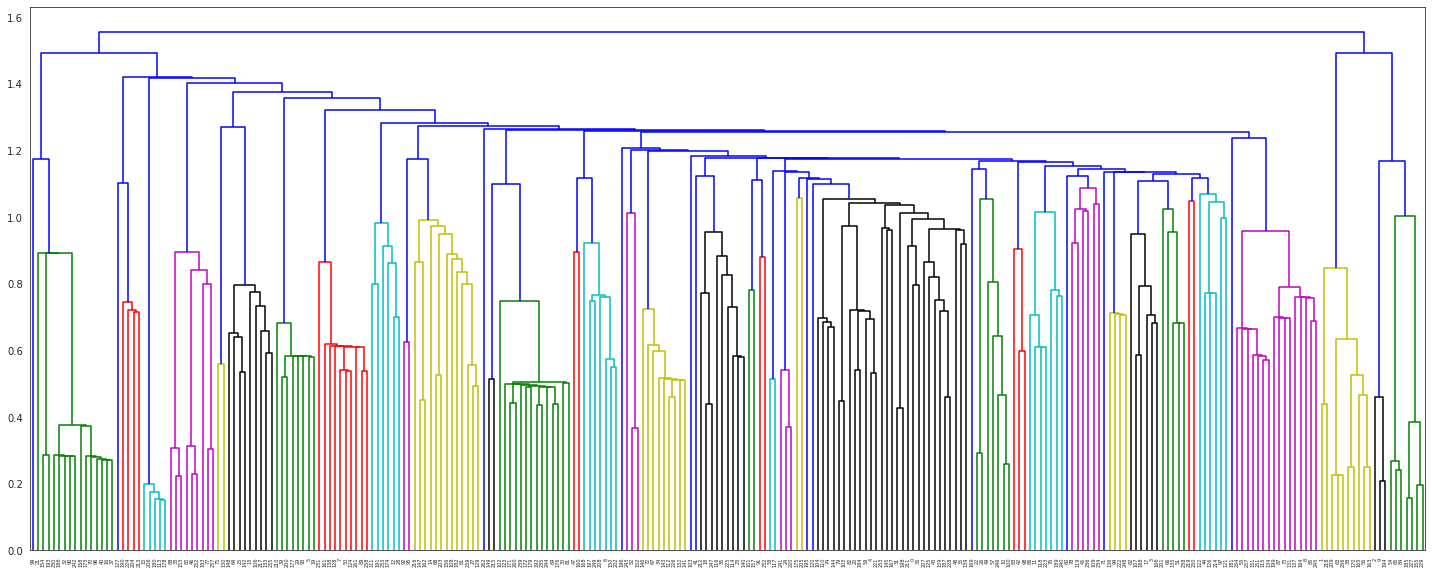
\includegraphics[width=\textwidth]{dendrogram.png}
  \caption{260 Filenames Clustered Using Cosine Similarity}
 \Description{260 Filenames Clustered using Cosine Simlilarity}
  \label{fig:teaser}
\end{teaserfigure}

%%
%% This command processes the author and affiliation and title
%% information and builds the first part of the formatted document.
\maketitle

\section{Introduction}
The purpose of generic data profiling is to produce metadata about one or more (usually many) datasets to discover general information about those datasets. In our case, for generic profiling, Task 1, we 
processed 1159 datasets. Our goal was to find the number of non-empty 
cells, number of empty cells, number of distinct values, the top-5 most 
frequent value(s), and the different data types
(integer, real, string and date-time). For different data types, we 
performed different statistical operations (min, max, most frequent values and so on). We were also tasked with identifying the
columns that are candidates for being keys of that specific table. 

The next step in understanding the dataset successfully is to study its underlying semantics. Semantic profiling enables us to gather knowledge
about the domain of
the data. If we are aware of what the domain of the data source is, we can 
profile it better and gain useful insights. For semantic profiling, Task 2,
we worked with a subset of Task 1's 1900 datasets; this subset consists of 260 columns from NYC Open Data datasets. We and identified and summarized the semantic types of these columns. For
different types, we used different methods to identify its types.
Regular Expressions and Patterns were used to identify phone number, website,
zip code, building
codes, locations, addresses, house numbers, school names, parks etc. These 
types are either very
distinct patterns e.g., phone number (ddd-ddd-dddd) or share a lot of similar
words. For example, most of the
street names have St, Ave and so on. For the types that don’t have these 
features like person names,
we took one of two approaches, depending on the type. For categories deemed
to contain mostly
distinct values but with context, we used Named-Entity Recognition (NER), 
Soundex and
natural language processing to label them. Otherwise, for sets with many 
repetitive items, we
generated Frequent Item Lists against which a given column’s row value can 
be compared. If the
item under consideration is in a given set, then the row containing that 
item is classified as the
set’s category. All code for this project can be viewed in the `develop' 
branch of this repository:
\url{https://github.com/theodorehadges/big_data_course_project/tree/develop/}.


\section{Methods}
\subsection{Task 1: Generic Profiling}

We imported all data as pyspark dataframes and used inferSchema() to narrow down the possible data types before classifying. If spark classifies a column as int, real, or date\_time then every row in that column is of that type. Otherwise, if there is one entry which is of a different type, spark will classify the whole column as a string. Therefore, if it it infers any type other than string, we can use that type as the classification. In most cases, this does not work since many columns are heterogeneous. Our next approach is to iterate through the columns of each file and perform builtin functions or use regex. Our main bottleneck is date\_time, since for high accuracy classifications of this type, many regex checks need to be made. We solve this by having three different date\_time checks ranging from low accuracy and fast to high accuracy and slow, and apply the most appropriate one for a given column given its size.

For task 1, we first iterate over every column for each data set in the NYC open data, and used
pyspark.sql.DataFrameReader(spark)’s InferSchema to check its data type.


This might return ['int', 'bigint', 'tinyint', 'smallint' ]for Integer type, ['float', 'double' , 'decimal'] for
Real type, ['timestamp', 'date', 'time', 'datetime'] for date\_time type and ['string'] for Text type.
However, since InferSchema will go over the column at once and if even one of the rows is ‘string’
or invalid value, it will return ‘string’ as the datatype for the whole column. So, just using
InferSchema wasn’t sufficient to identify the column types that might be dirty or have multiple
data types and invalid values or outliers.

For Integer, Real and Date\_Time(timestamp) returned by inferSchema(), we compute the relevant
statistics using Spark SQL.

Next, we selected the ‘string’ type columns returned by the inferSchema() and tried to
interpret these particular columns as int, real and date\_time and strings by performing explicit type
casting. If it can be returned as these three types, we return that type’s object, if not, we keep it as
string and move to the next item for interpretation. This entire process is applied using Spark UDFs
so it is distributed. 

Specifically, for date\_time and string types, we had three different versions of methods to interpret
and parse their values since the formats of date and time can vary greatly. Using libraries
such as Python’s dateutil.parser is not accurate as it can result in false positive date\_time
interpretation, skewing our understanding of the data.





\subsection{Task 2: Semantic Profiling}
For task 2, our approach can be divided into three parts for finding different semantic types:
\begin{enumerate}
    \item Regex for checking types with very distinct patterns; e.g., phone number(ddd-ddd-dddd) 
    \item Named-entity recognition (NER) and natural language processing for checking types that don’t have a distinct pattern or similar words but can be identified with NER tags. The SpaCy implementation ‘en\_core\_web\_md’ has been used. This technique is used for
    identifying cities and people’s names. The PERSON and GPE tags were used.
    \item Comparing row values against frequent item lists, where those lists contain the most
frequent items for each category. If a row value is contained in the frequent item list, then
the row is classified as the category from which the frequent item list was derived. This is
a useful approach when there are many repeated values in a category.
\end{enumerate}
For each method, we defined different functions to identify different types, and in the function we
return the percentage of how many rows were identified as such types, if it’s larger than a certain
threshold, we return the found\_type and total count of rows that identified as such type.


\subsubsection{Method 1:Regex}

The following semantic data types were found using regex. We found this to be a suitable approach for types such as these, which have either an identifiable format (five ints suggests zipcode), or a few key words like HS, Academy, and School for the school\_name category.
\begin{itemize}
    \item Phone number
    \item website
    \item zip code
    \item building code
    \item lat lon
    \item street
    \item address
    \item school name
    \item house number
    \item school subjects
    \item school level
\end{itemize}

This seemed like a viable approach for this set of categories. However, Street and Address were tricky in that these two types share many similar words such as Road, Street, St, Ave and so on. Therefore, during the execution, they were always labeled together. In observing the data, we noticed that address types usually are longer than street names in length. Therefore, to solve the problem of Street and Address being indistinguishable, we compute the average length for all the columns. We tested and found optimal thresholds: if the string is less than or equal to 15 characters, it's a street; otherwise, it is an address. In this way, we successfully distinguished these two types. \newline 

\subsubsection{Method 2:Named Entity Recognition (NER) and Soundex}
The following semantic data types were found using NER and Soundex:
\begin{itemize}
    \item city (NER)
    \item person name (NER)
    \item car make
    \item car model
    \item color
\end{itemize}

Named Entity Recognition is one of the sub-tasks of information retrieval. It can be used to identify various information regarding the semantics of the text. It can give information about people, places, time, quantities, money, organizations, and more. We employed the Spacy implementation of NER in Task 2 to identify people and cities. The people have been identified using the PEOPLE tag and the cities have been identified using the GPE (Geo Political Entity) tag.

Soundex has been used to identify similar or phonetically similar sounding words. This is a good approach for identifying the color names and the car makers. It helps in converging the misspelled words together. 

\subsubsection{Method 3: Similarity and Frequent Item Comparison}
The following semantic data types were found using Similarity and Frequent Item Comparison:
\begin{itemize}
    \item business names
    \item areas of study
    \item city agency
    \item location type
    \item school subject
    \item parks & playgrounds
\end{itemize}

The pipeline for this method is as follows: First, we need to determine the categories of each file. To achieve this, we decided to group similar files together. In similarity.py, we used file names as a proxy for file content similarity and applied cosine similarity with 3-grams onto the filenames to create a m x m similarity matrix, where m is the list of filenames (Fig 2). In the figure similar files are represented by a bright dot where the higher their similarity, the brighter the dot. Thus, the presence of some bright dots in the similarity matrix motivated us to find out if files could be clustered by file name.

\begin{figure}[h]
  \centering
  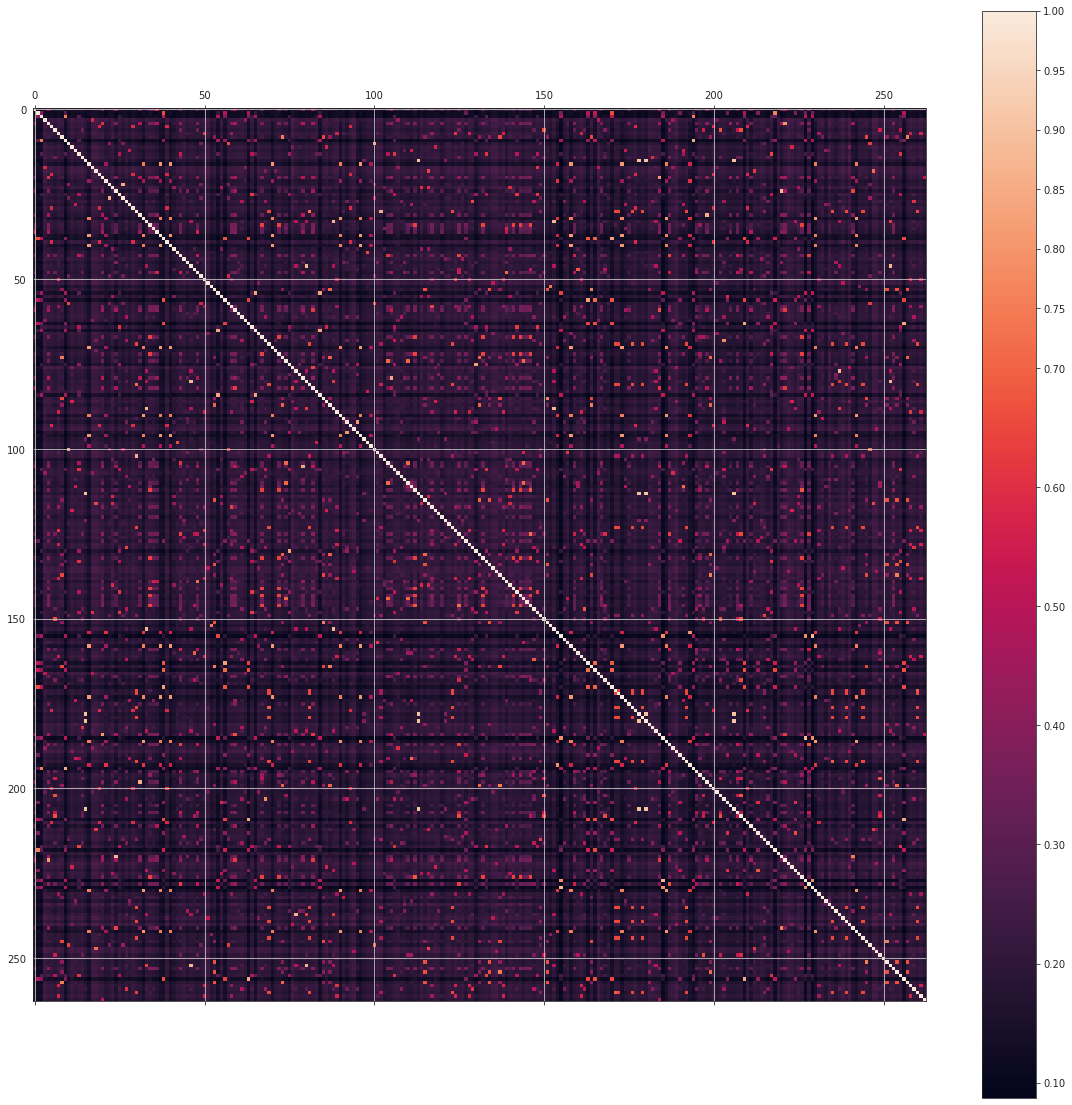
\includegraphics[width=\linewidth]{similarity.png}
  \caption{Filename n x n Cosine Similarity Matrix. The presence of some bright (similar)
dots in the similarity matrix motivated us
to find out if files could be clustered by file
name.}
  \Description{Filename n x n Cosine Similarity Matrix. The presence of some bright (similar)
dots in the similarity matrix motivated us
to find out if files could be clustered by file
name.}
\end{figure}


We passed the similarity matrix into the scipy cluster hierchy linkage() function to generate a linkage matrix, Z. Finally, Z was passed into scipy’s fcluster() function to form flat clusters from Z. We made a simple python dictionary using the resulting fcluster structure with key value pairs: clusterN: [filenameR, filenameS], where all filenames in clusterN are similar. 

\begin{figure}[h]
  \centering
  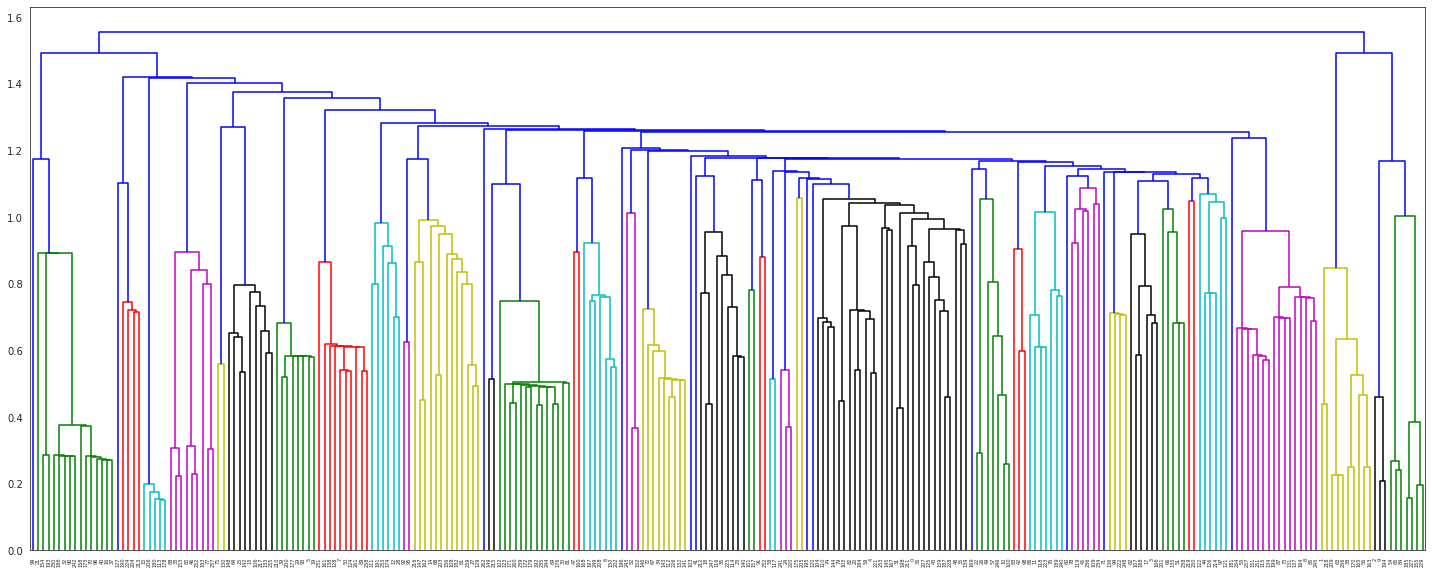
\includegraphics[width=\linewidth]{dendrogram.png}
  \caption{Linkage Matrix. The vertical lines in this dendrogram represent filenames. Neighbored lines were mapped to same cluster.}
  \Description{Linkage Matrix Dendrogram}
\end{figure}

In Figure 3, Vertical lines represent filenames. Neighbored lines (color-coded) were mapped to same cluster. The lower portions represent the resulting files which were mapped to the same clusters. As you can see (from their similar heights), many file names were correctly mapped to clusters containing files with similar file names. We wrote this final dictionary to a JSON file.

Next, once the file names were clustered we identified files which were mapped to the same clusters as being the same type. Of course, since this clustering was unsupervised, it was not perfectly clustered. However, we were lucky in that all of the data types we set out to classify for this part were mapped to homogeneous clusters. In generate\_keyword\_lists\_from\_columns.py, we use the file clusters to generate the most frequent items in each. Each file in the cluster is loaded into a dataframe. Each row in the data frame is exploded such that each word is now in its own row. This is useful so that we can perform some filtering.

For every file in the cluster, we take the most frequent n words (n depends on category) and union it with the n most frequent values of the next file’s most frequent n words. This results in a concise set which is representative of the majority of that category (assuming there are many repeat items in that category). We manually removed some list entries which may be present in another category to avoid ambiguity; however, this could also have been done by finding the intersection of all category sets and removing the resulting values from each set.
 
Finally, in task2.py, we use these frequent item lists to check if values in a given row contain any of the items in the frequent itemset for each category. If it does, then that row is classified as the type from which the itemset was derived.

\section{Results}
\subsection{Task 1: Results}
The first thing to notice is that by looking at Figure 4 and Figure 5 we can see that most data is classified as either integer or text. However, upon performing much more precise and resource intensive mining, it may be possible to extract more Date/Time data from the Text fields. Below, in Table 1 and Table 2, we can see the raw values from which the diagrams were derived.

In Figure 6, we can see that most of the data, about 82\%, contained values, while the remaining 18\% contained empty data cells.

%\begin{table*}
\begin{table}[h]
  \caption{Number of Columns with Identified Types}
  \label{tab:commands}
  \begin{tabular}{ccl}
    \toprule
    Type & Count\\
    \midrule
    \texttt{INTEGER (LONG)} & 11674 \\
    \texttt{TEXT} & 13646\\
    \texttt{DATE/TIME} &1137\\
    \texttt{REAL} & 4527\\
    \bottomrule
  \end{tabular}
\end{table}
%\end{table*}

%\begin{table*}
\begin{table}[H]
  \caption{Number of Cells with Identified Types}
  \label{tab:commands}
  \begin{tabular}{ccl}
    \toprule
    Type & Count\\
    \midrule
    \texttt{INTEGER (LONG)} & 675048313 \\
    \texttt{TEXT} & 957412154 \\
    \texttt{DATE/TIME} & 405729706\\
    \texttt{REAL} & 435655955\\
    \bottomrule
  \end{tabular}
\end{table}
%\end{table*}

\begin{figure}[h]
  \centering
  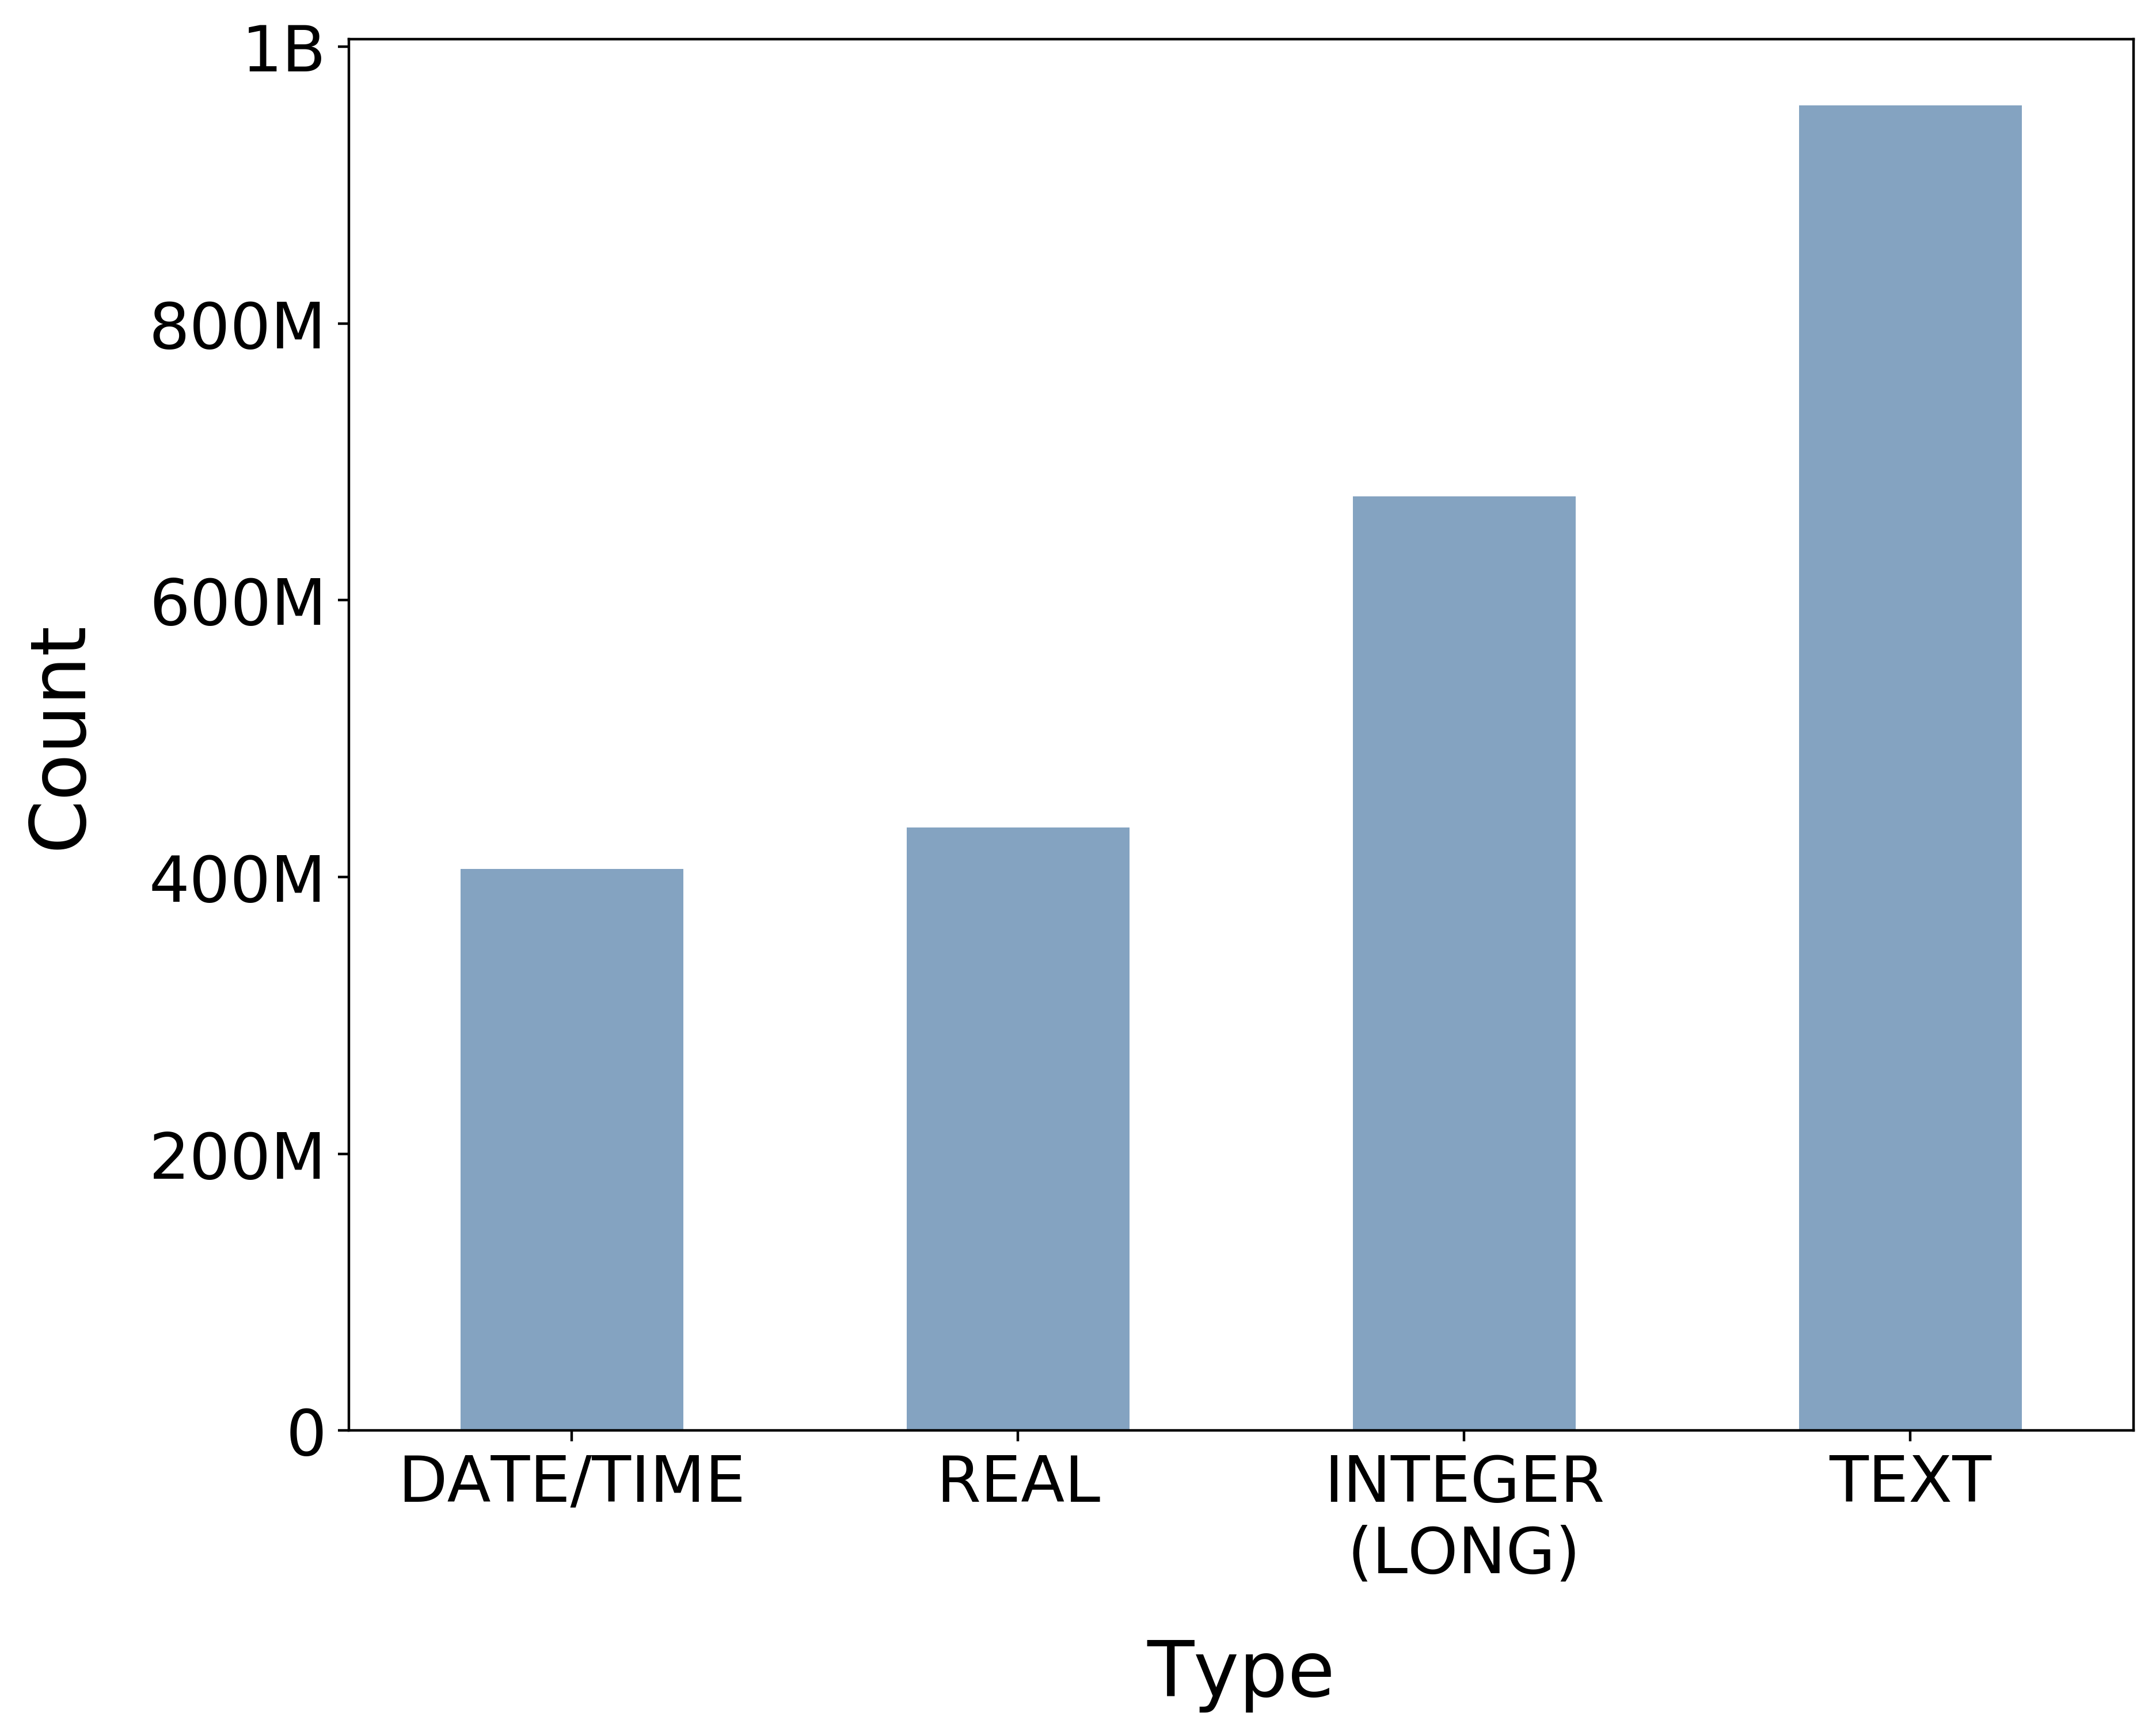
\includegraphics[width=\linewidth]{tot_cols_for_each_type.png}
  \caption{Total Number of Columns for Each Type}
  \Description{Total Number of Columns for Each Type}
\end{figure}



\begin{figure}[h]
  \centering
  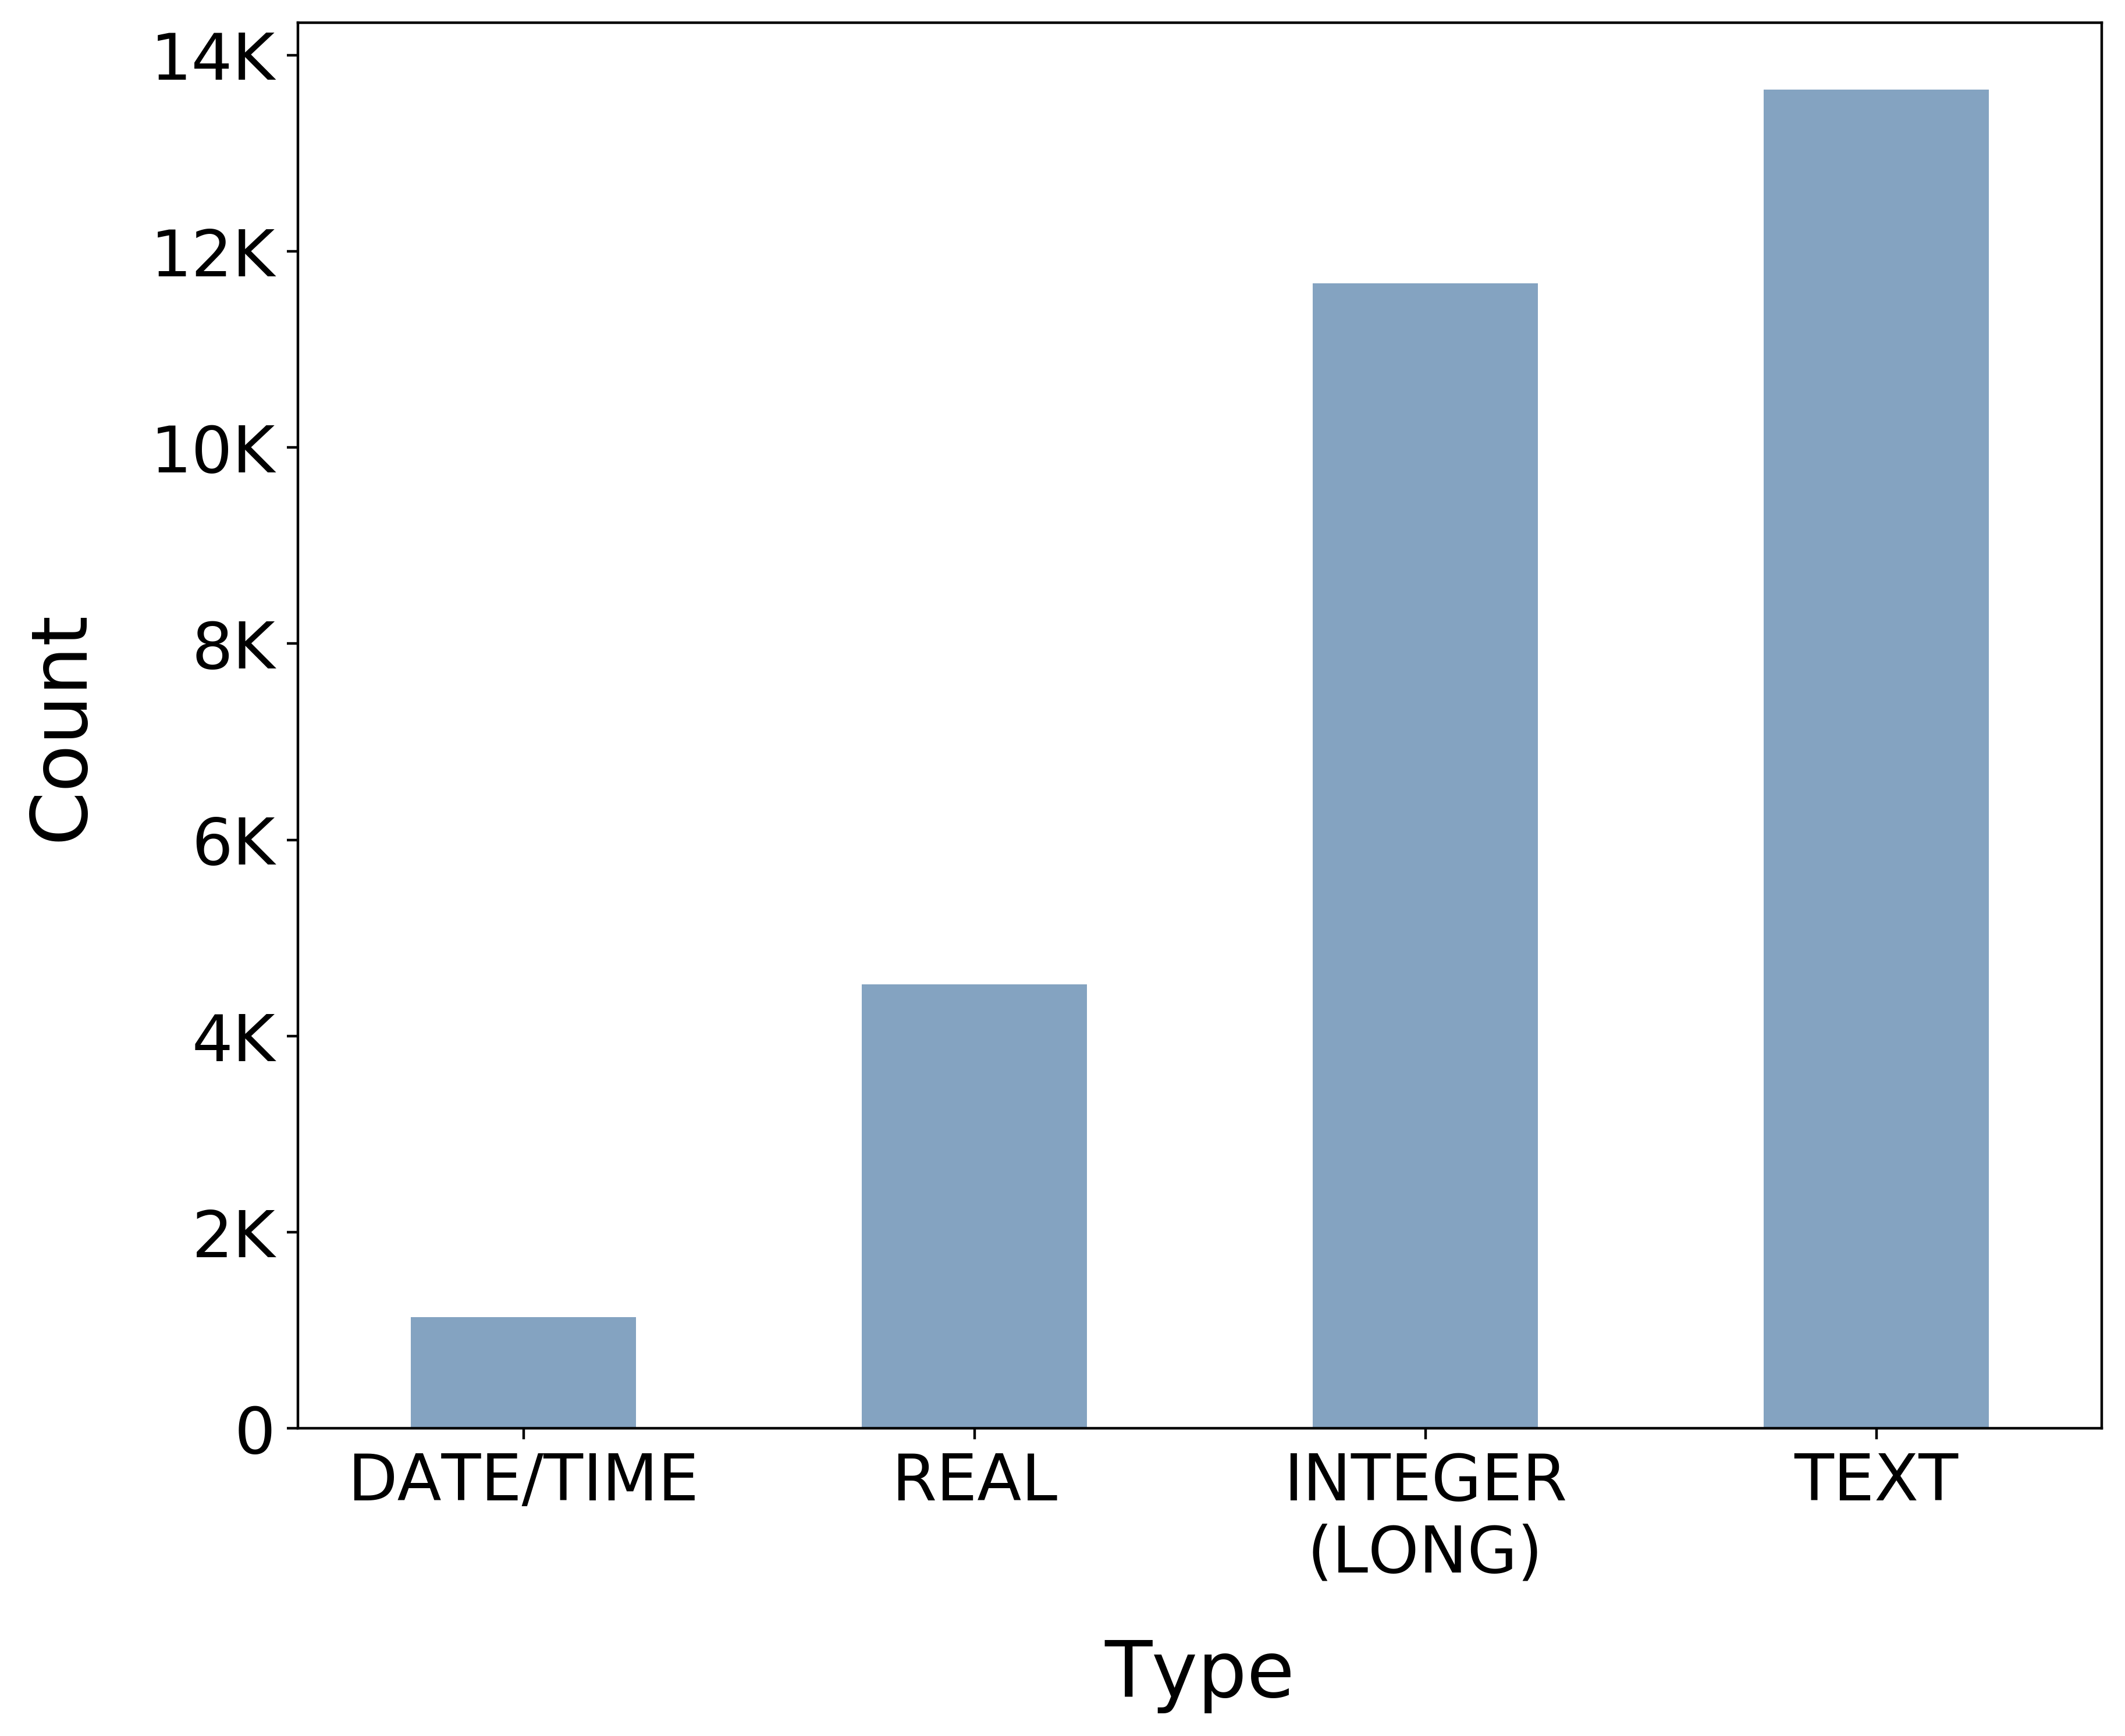
\includegraphics[width=\linewidth]{tot_cells_for_each_type.png}
  \caption{Total Number of Cells for Each Type}
  \Description{Total Number of Cells for Each Type}
\end{figure}

In Table 3, we can see a summary of the 1159 datasets. One thing to observe is that the empty cells row has a median of 0.0 and a mode of 0. Therefore it must be the case that most of the datasets do not have empty cells.


\begin{table*}
%\begin{table*}[t]\setlength\tabcolsep{5pt}
  \caption{\textbf{Quantitative Summary of Task 1 Results}}
  %\label{tab:commands}
  %\begin{tabular}{ccl}
 \begin{tabular}{| l | l | l | l | l | l | l | l}
    \toprule
    \thead{\textbf{Type}} &\textbf{Mean} & \textbf{std} &\textbf{mincount} &  \textbf{maxcount} & \textbf{median} & \textbf{mode} \\
    \midrule
    \textbf{empty cells} & 20682.11 & 336203.51 & 0 & 16385532 & 0.0 & 0\\
    \textbf{non-empty cells} & 94945.66 & 1150276.58 & 0 & 50846562 & 1381.0 & 0 \\
    \textbf{distinct values} & 8389.23 & 201663.02 & 0 & 12099654 & 33.0 & 2\\
    \bottomrule
  \end{tabular}
\end{table*}


Finally, we observed candidate key. The results are shown in Table 4. We found datasets with the largest potential and smallest potential candidate key. 587 datasets don’t have a candidate key, hence a composite key or indexing is required
%\begin{table*}
\begin{table}[H]
  \caption{Candidate Key Counts}
  \Description{test}
  \label{tab:commands}
  \begin{tabular}{ccl}
    \toprule
    Type & Count\\
    \midrule
    \texttt{Largest} & 255 \\
    \texttt{Average} & 2.55\\
    \texttt{Lowest} & 0\\
    \texttt{Number of datasets without keys} & 587\\
    \bottomrule
    \multicolumn{2}{l}{\footnotesize 587 datasets do not have a candidate key; composite/index may be required.}\\
    %\Description{test}
  \end{tabular}
\end{table}
%\end{table*}


\begin{figure}[h]
  \centering
  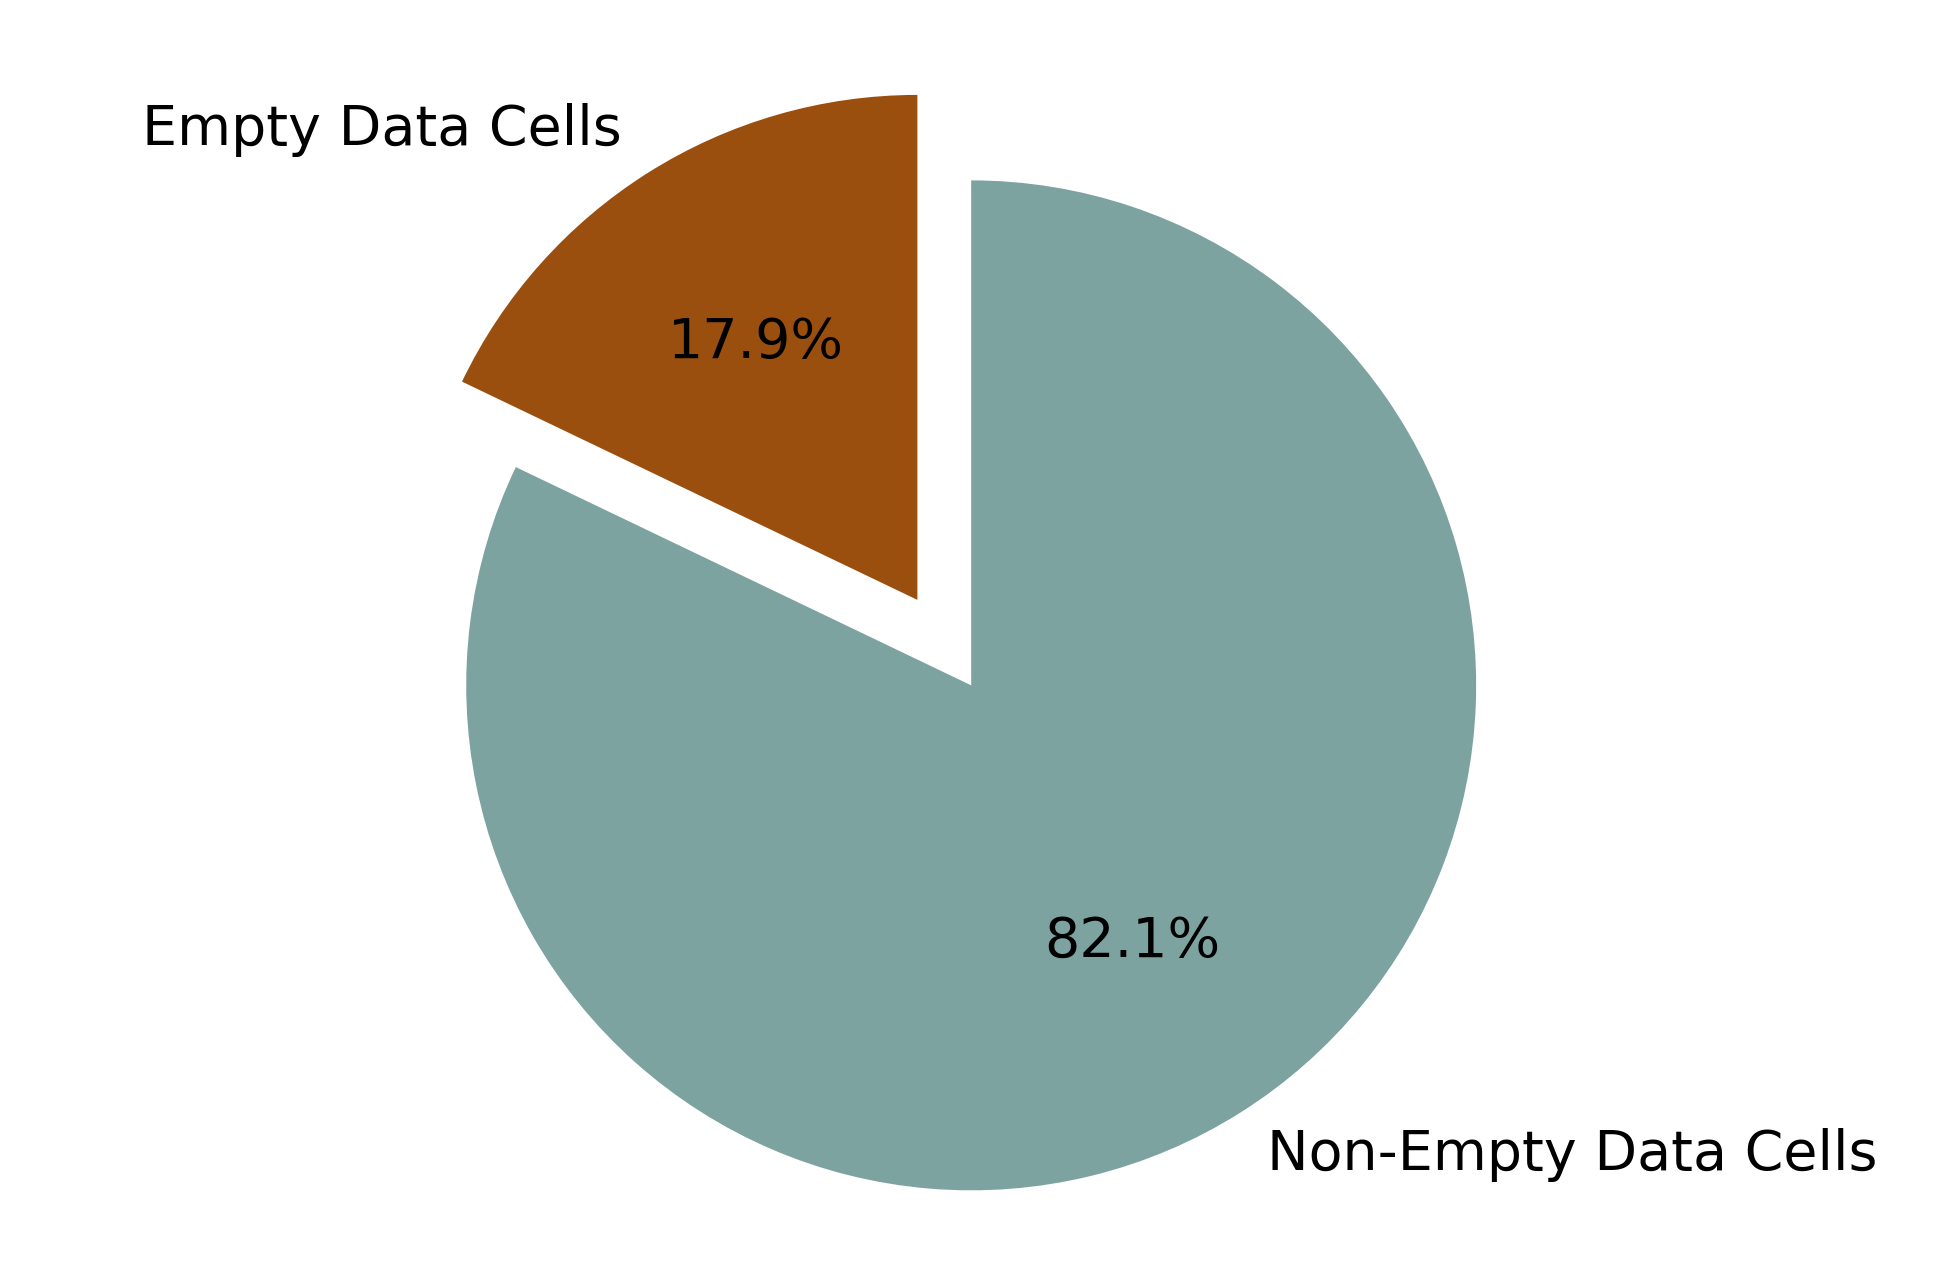
\includegraphics[width=\linewidth]{avg_completeness_no_title.png}
  \caption{Average Completeness of Data}
  \Description{On average, 82\% of the cells in a given dataset are non-empty.}
\end{figure}



\subsection{Task 2: Results}

The dataset was manually labelled and then the semantic classification of the columns from various datasets were performed. A list of the 23 most suitable labels was created for the datasets, as shown n Figure 7. An average recall of 71.38\% was seen and an average precision of 72.40\% was observed.
\begin{figure}[H]
  \centering
  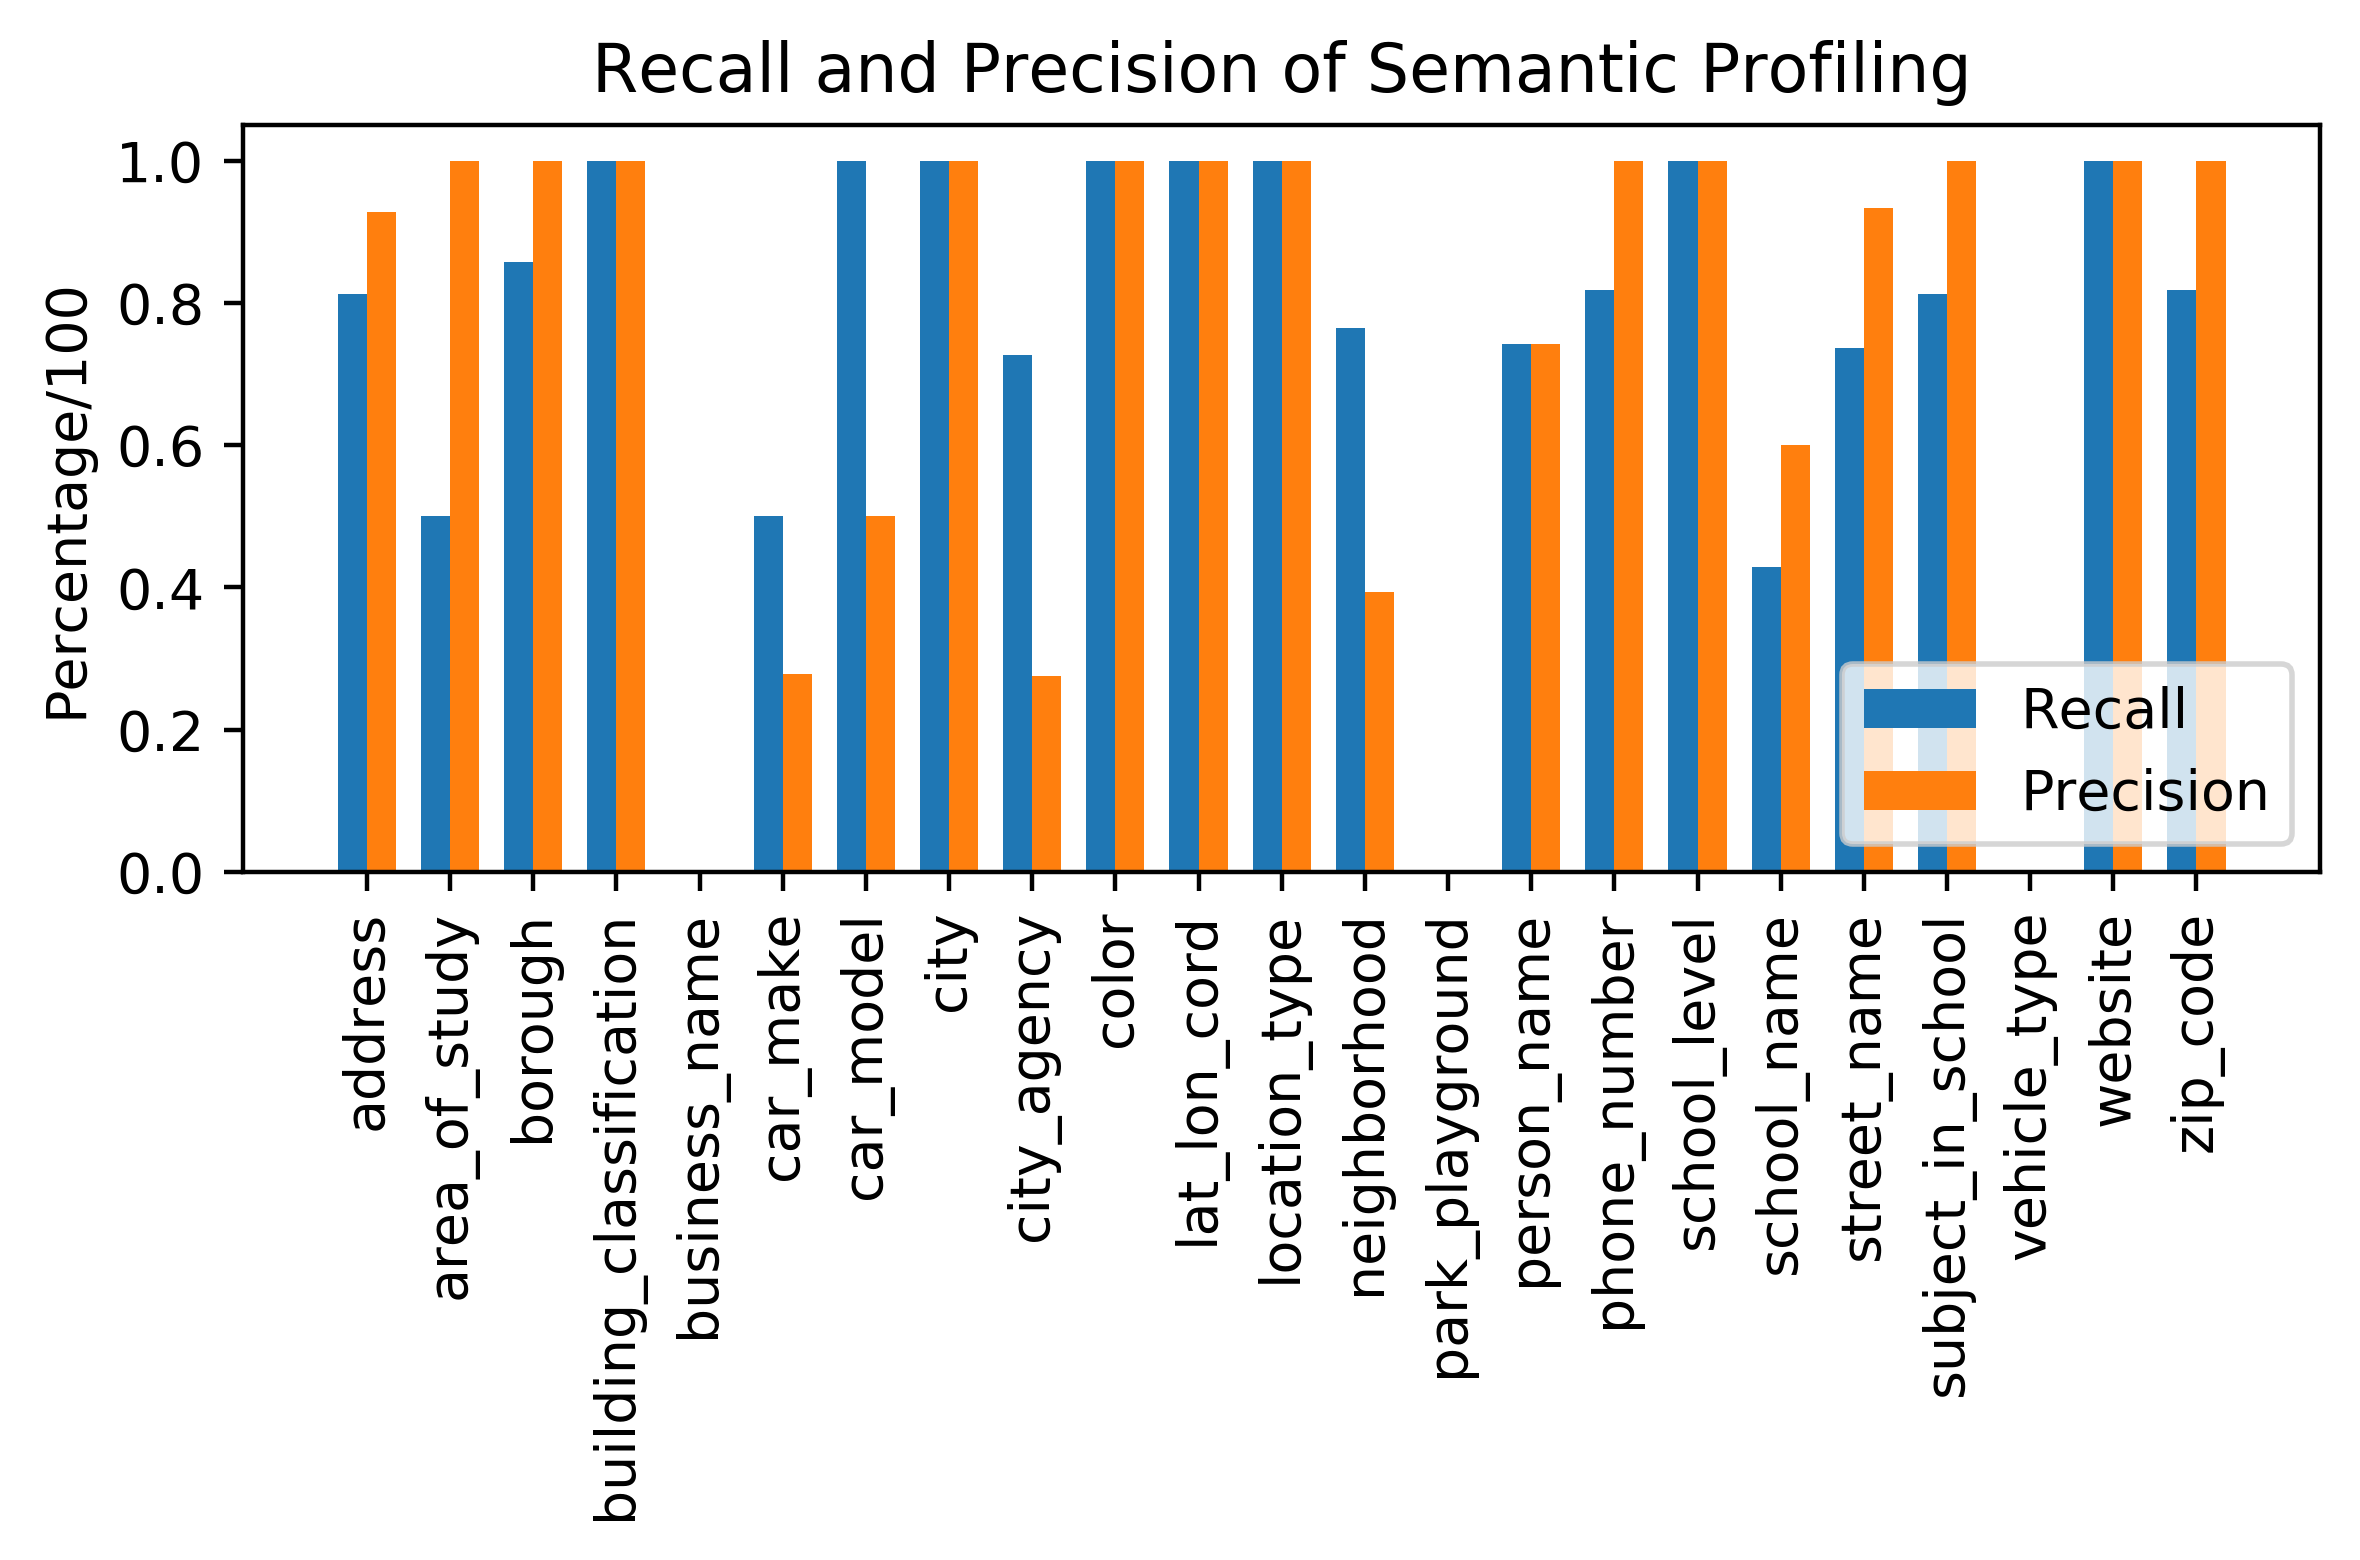
\includegraphics[width=\linewidth]{precision_recall.png}
  \caption{Recall and Precision of Semantic Profiling}
  \Description{On average, 82\% of the cells in a given dataset are non-empty.}
\end{figure}

\section{Challenges and Optimizations}
\subsection{Task 1: Challenges and Optimizations}
At the very beginning stage of the project, we tried iterating over all the columns of the dataset (row wise). But this resulted in an extremely slow script because of losing the Spark scalability to sequential execution. 
 
To solve this problem, the Spark dataframes and RDDs were strictly used for processing. Further, another problem arose: (1) using inferSchema() has a limit in identifying columns with multiple values (2) date\_time type has many different formats, so it’s hard to distinguish them from strings , we tried to iterate every cell and check its types using regex. However, after executing a few files, we soon realized this method will be too time consuming as it has to iterate every value and compare it to four different regex lists. 

Then, we come up with the idea of trying to interpret values in all the columns which have a return type of ‘string’ after implementing inferSchema(). However, we faced the third problem (3) using library to parse the date\_time might be fast but it’s not as accurate as checking with a regex list, but checking regex list will be too time consuming especially for large data-sets. (We have about 6 data sets that’s larger than 1 GB). So we came up with three versions of interpreting sting and date\_time:
\begin{enumerate}
    \item Use Python’s dateutil.parser, which is low accuracy but high speed.
    \item Use both Python’s dateutil.parser and a single regex check, which is of moderate speed and accuracy.
    \item Use both dateutil.parser a list of more well-defined regex, which is low speed but high accuracy.
\end{enumerate}

The idea behind this is to execute different sizes of data-sets using different methods, for larger data-sets, we switched to the (1) method and for smaller data-sets, we used (2) or (3) methods. In that way, we managed to find a balance between the speed and accuracy which we think is also applicable for other applications and projects.  


\subsection{Task2: Challenges and Optimizations}
\subsubsection{NLP and NER}
The biggest challenge for NER implementation was the inability to perform NLP in a distributed manner due to infrastructural restrictions of the Dumbo platform. To use NLP toolkits like SpaCy and NLTK in a distributed manner, these libraries must be installed on each of the worker nodes. Doing so with restricted permissions or with custom environment was not possible so a sequential approach had to be taken.

There were some key decision making steps involved in making the best use of Spacy NER. During the initial trials we made use of the available en\_core\_web\_sm 2.0, the semantic parser trained on a small web dataset that was available on the Dumbo Python 3.6.5 module. However, this being an outdated version, we made use of a custom  environment with en\_core\_web\_md 2.2 version of the parser which is trained on a much bigger and newer web datasets. There was a significant improvement in the results. With the en\_core\_web\_sm 2.0 the word hits for NER were as low as 10-20\%. With en\_core\_web\_md 2.2, this rate increased to as low as about 40\% of the words being mapped and as high as 70-80\% words getting mapped.

The key decision making step with a sequential approach to NER was to choose the trade-off between precision and execution time. Initially we tried to improve times for sampling. However, sampling is prone to not being representative of the entire data so we decided to discard this approach. Since, we were working on much smaller datasets, we chose to trade-off higher execution times for higher precision by using the sequential processing approach. The best solution to this would have been applying NLP in a distributed manner.

\subsubsection{Similarity and Frequent Item Comparison}
We start this task by looking for easily classifiable categories such as city agency. We observed the data for city agency and noticed that it was very clean in that it does not contain any extra characters, and it is very similar to the official data on the nyc.gov website. Therefore we built a simple scraper, nyc\_agency\_scraper.py using BeautifulSoup and parsed the string names of an agency to one file and the abbreviations of that agency to another file. The idea was that we could do a simple contains() to see if a value is contained in this list. We moved on to other types in this section and realized that using sources such as these would be great for general classification, but since we can observe our datasets, there might be a smarter way to choose the list to compare against. 
 
By smarter, we mean a smaller list which yields higher accuracy. We started observing the datasets and skimming through to see items which seemed frequent and made lists for comparison. However, we realized that this is not a scalable solution for building representative itemsets and took a step back. We generated the aforementioned similarity matrix, performed clustering, and built a list generator for frequent items for each category across all files in that category. File name clustering was not perfect at first. After writing a function for jaccard similarity and experimenting with different shingle sizes, we found that 3-grams worked best. However, the clustering was not ideal. We later found a cosine similarity function and were happy to find that the results were much better. After reading about it, we learned that cosine similarity tends to be a better metric than jaccard when measuring similarity between text sets. One challenge we still face is that we would like to use frequent itemsets of size 2 or 3 in some cases (rather than just a frequent itemset of singletons). In the future, we plan on adding this functionality so that we can have better accuracy during the row classification step.

\section{Individual Contributions}
\subsection{Task 1: Generic Profiling}
\textbf{Ankush Jain}: 
\begin{itemize}
    \item Built data pipeline
    \item String data interpretation
    \item Code optimization
\end{itemize}
\textbf{Theodore Hadges}: 
\begin{itemize}
    \item Generic profiling
    \item Integer profiling
    \item Real profiling
\end{itemize}
\textbf{Ruinan Zhang:}
\begin{itemize}
    \item String profiling
    \item Date\_time profiling
    \item RegEx-based filtering functions
\end{itemize} 

\vfill\null
\columnbreak

\subsection{Task 2: Semantic Profiling}
\textbf{Ankush Jain}: 
\begin{itemize}
    \item Named Entity Recognition classification
    \item Soundex classification
    \item Categories:
    \begin{itemize}
        \item person\_name
        \item city
        \item color
        \item car\_make
        \item borough
    \end{itemize}
\end{itemize}
\textbf{Theodore Hadges}: 
\begin{itemize}
    \item Cluster analysis
    \item Frequent item classification
    \item Categories:
    \begin{itemize}
        \item area\_of\_study
        \item neighborhood
        \item city\_agency
        \item location\_type
        \item parks
        \item businesses\_name
    \end{itemize}
\end{itemize}
\textbf{Ruinan Zhang:}
\begin{itemize}
    \item Built data pipeline
    \item RegEx classification
    \item Categories:
    \begin{itemize}
        \item address
        \item street
        \item website
        \item phone
        \item lat\_lon\_coord
        \item building\_class
        \item zip code
        \item school\_subjects
    \end{itemize}
\end{itemize}


%A ``teaser figure'' is an image, or set of images in one figure, that
%are placed after all author and affiliation information, and before
%the body of the article, spanning the page. If you wish to have such a
%%figure in your article, place the command immediately before the
%\verb|\maketitle| command:



 


%%
%% The acknowledgments section is defined using the "acks" environment
%% (and NOT an unnumbered section). This ensures the proper
%% identification of the section in the article metadata, and the
%% consistent spelling of the heading.
\begin{acks}
Thank you to Professor Julia Stoyanovich and Professor Juliana Freire for tasking us with this project. Our freedom to explore and experiment with different methods made for a challenging journey yet we are grateful to have had an opportunity to have such freedom; after all, the benefit of one taking a breadth-first path toward a leaf-node destination is that one learns something new at each node visited.
\end{acks}

%%
%% The next two lines define the bibliography style to be used, and
%% the bibliography file.
\bibliographystyle{ACM-Reference-Format}
    %\bibliographystyle{ACM-Reference-Format}
    \bibliography{sample-bib}
%\bibliography{sample-bib}
\nocite{Ramaswamy:2000:EAM:342009.335437}
\nocite{Chandola:2009:ADS:1541880.1541882}
\nocite{Hua:2007:CDM:1281192.1281294}
\nocite{Ester:1996:DAD:3001460.3001507}
\end{document}
\endinput
%%
%% End of file `sample-authordraft.tex'.
